\documentclass[11pt, a4paper]{article}
\usepackage{pdfpages}
\usepackage{parallel}
\usepackage[T2A]{fontenc}
%\usepackage{ucs}
\usepackage[utf8]{inputenc}
\usepackage[english,russian]{babel}
\usepackage{hyperref}
\usepackage{rotating}
\usepackage[inner=2cm,top=1.8cm,outer=2cm,bottom=2.3cm,nohead]{geometry}
%\usepackage{listings}
\usepackage{graphicx}
\usepackage{wrapfig}
\usepackage{longtable}
\usepackage{indentfirst}
\usepackage{array}
\usepackage{tikzsymbols}
\usepackage{soul}
\usepackage[ruled,vlined]{algorithm2e}
\usepackage{qrcode}
\counterwithout{figure}{section} 

\usepackage{url}
\makeatletter
\g@addto@macro{\UrlBreaks}{\UrlOrds}
\makeatother

\newcolumntype{P}[1]{>{\raggedright\arraybackslash}p{#1}}
\frenchspacing
%\usepackage{fixltx2e} %text sub- and superscripts
\usepackage{icomma} % коскі ў матэматычным рэжыме
%\PreloadUnicodePage{4}

\newcommand{\longpage}{\enlargethispage{\baselineskip}}
\newcommand{\shortpage}{\enlargethispage{-\baselineskip}}

\def\switchlang#1{\expandafter\csname switchlang#1\endcsname}
\def\switchlangbe{
\let\saverefname=\refname%
\def\refname{Літаратура}%
\def\figurename{Іл.}%
}
\def\switchlangru{
\let\saverefname=\refname%
\let\savefigurename=\figurename%
\def\refname{Литература}%
\def\figurename{Рис.}%
}
\def\switchlangen{
\let\saverefname=\refname%
\def\refname{References}%
\def\figurename{Fig.}%
}

\hyphenation{admi-ni-stra-tive}
\hyphenation{ex-pe-ri-ence}
\hyphenation{fle-xi-bi-li-ty}
\hyphenation{Py-thon}
\hyphenation{ma-the-ma-ti-cal}
\hyphenation{re-ported}
\hyphenation{imp-le-menta-tions}
\hyphenation{pro-vides}
\hyphenation{en-gi-neering}
\hyphenation{com-pa-ti-bi-li-ty}
\hyphenation{im-pos-sible}
\hyphenation{desk-top}
\hyphenation{elec-tro-nic}
\hyphenation{com-pa-ny}
\hyphenation{de-ve-lop-ment}
\hyphenation{de-ve-loping}
\hyphenation{de-ve-lop}
\hyphenation{da-ta-ba-se}
\hyphenation{plat-forms}
\hyphenation{or-ga-ni-za-tion}
\hyphenation{pro-gramming}
\hyphenation{in-stru-ments}
\hyphenation{Li-nux}
\hyphenation{sour-ce}
\hyphenation{en-vi-ron-ment}
\hyphenation{Te-le-pathy}
\hyphenation{Li-nux-ov-ka}
\hyphenation{Open-BSD}
\hyphenation{Free-BSD}
\hyphenation{men-ti-on-ed}
\hyphenation{app-li-ca-tion}

\def\progref!#1!{\texttt{#1}}
\renewcommand{\arraystretch}{2} %Іначай формулы ў матрыцы зліпаюцца з лініямі
\usepackage{array}

\def\interview #1 (#2), #3, #4, #5\par{

\section[#1, #3, #4]{#1 -- #3, #4}
\def\qname{LVEE}
\def\aname{#1}
\def\q ##1\par{{\noindent \bf \qname: ##1 }\par}
\def\a{{\noindent \bf \aname: } \def\qname{L}\def\aname{#2}}
}

\def\interview* #1 (#2), #3, #4, #5\par{

\section*{#1\\{\small\rm #3, #4. #5}}
\ifx\ParallelWhichBox\undefined%
    \addcontentsline{toc}{section}{#1, #3, #4}%
\else%
\ifnum\ParallelWhichBox=0%
    \addcontentsline{toc}{section}{#1, #3, #4}%
\fi\fi%

\def\qname{LVEE}
\def\aname{#1}
\def\q ##1\par{{\noindent \bf \qname: ##1 }\par}
\def\a{{\noindent \bf \aname: } \def\qname{L}\def\aname{#2}}
}

\newcommand{\interviewfooter}[1]{
\vskip 1em
\noindent \textit{#1}
}

\AtEndDocument{\vfill\centering \qrcode{https://github.com/fiowro/mouses/blob/main/\jobname.pdf}}

\switchlang{ru}
\begin{document}

\title{1987 "--- Genius GM-5 mouse}
\date{}
\maketitle
\selectlanguage{russian}

Мышь GM-5 была выпущена тайваньской компанией KYE Systens (владельцем торговой марки  Genius) для использования с компьютерами Commodore 64 (первыми домашним компьютерами массового производства, выпускавшимися с 1982 по 1992 год). Датировку мыши можно выполнить на основании рекламы KYE Systems, в которой упоминаются модели GM-2 (мышь, произведенная Z-Nix в 1986 году и продававшаяся под несколькими брэндами), GM-3 (первая  мышь, произведенная KYE самостоятельно, в <<новом>> относительно GM-2 корпусе, с последовательным интерфейсом и внешним питанием), а также аналогичная GM-4 без дополнительного питания \cite{YourComputer}. Модель GM-6 в ещё более новом корпусе с широкими плоскими кнопками, ставшая первой по-настоящему массовой мышью Genius (и заодно первой мышью Genius с зарегистрированным FCC ID), датируется 1987 годом, а её модификация GM-6000 - 1988. Таким образом, мышь GM-5 фактически представляет собой чуть более позднюю модификацию GM-3, выполненную для компьютеров Commodore, и могла появиться либо в конце 1986, либо, что более вероятно, в 1987 году.

\begin{figure}[h]
   \centering
    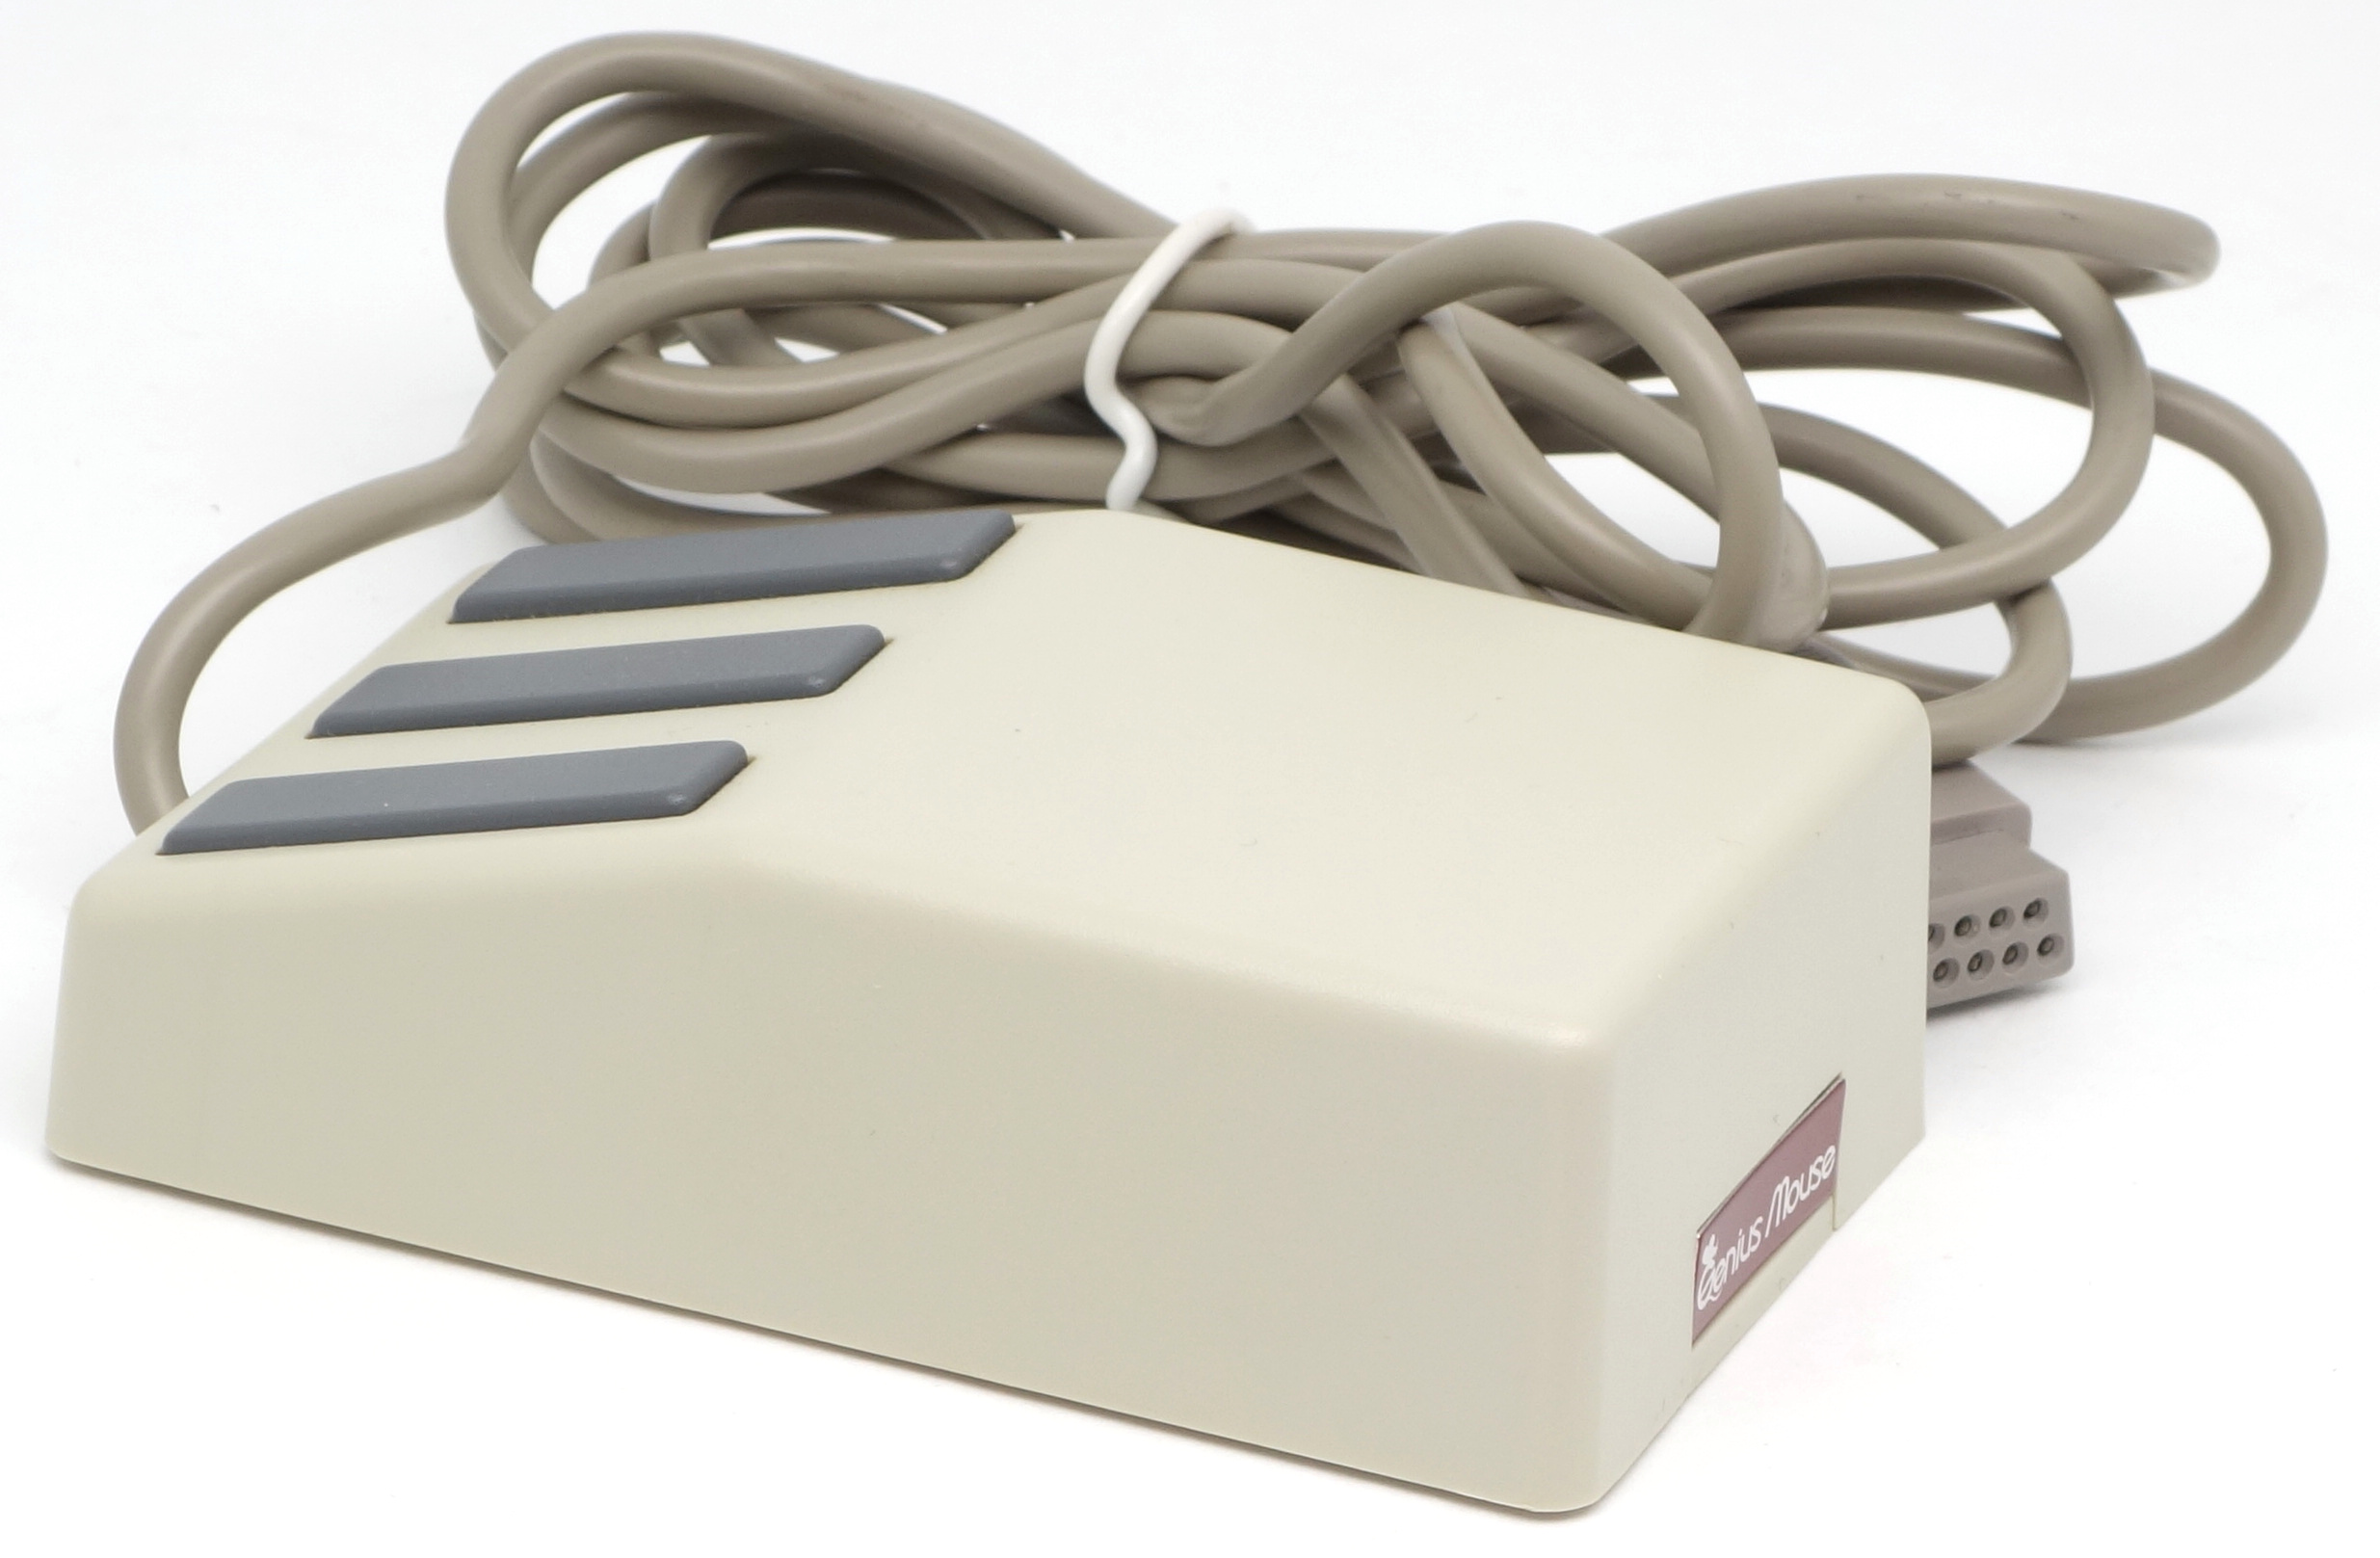
\includegraphics[scale=0.77]{1987_genius_gm5_mouse/pic_30.jpg}
    \caption{Genius GM-5}
    \label{fig:GM5MousePic}
\end{figure}

Мышь выполнена в бежевом корпусе, демонстрирующем строгий индустриальный дизайн и минимализм. Корпус имеет практически прямоугольную форму, если не считать скошенную вперёд часть верхней грани, на которой находятся три вытянутые прямоугольные кнопки серого цвета. Кабель мыши не снабжен ограничительной втулкой, которая защищала бы его от механических повреждений в месте выхода из корпуса. На нижней стороне (рис. \ref{fig:GM5MouseTopAndBottom}) присутствует съемное кольцо из контрастного серого пластика, позволяющее извлечь шар для чистки мыши (оно крепится шурупом --- конструкция, характерная для мышей первой половины 80-х годов). Также на нижней стороне присутствуют три дополнительных металлических шарика, играющих роль опор с низким коэффициентом трения.

\begin{figure}[h]
    \centering
    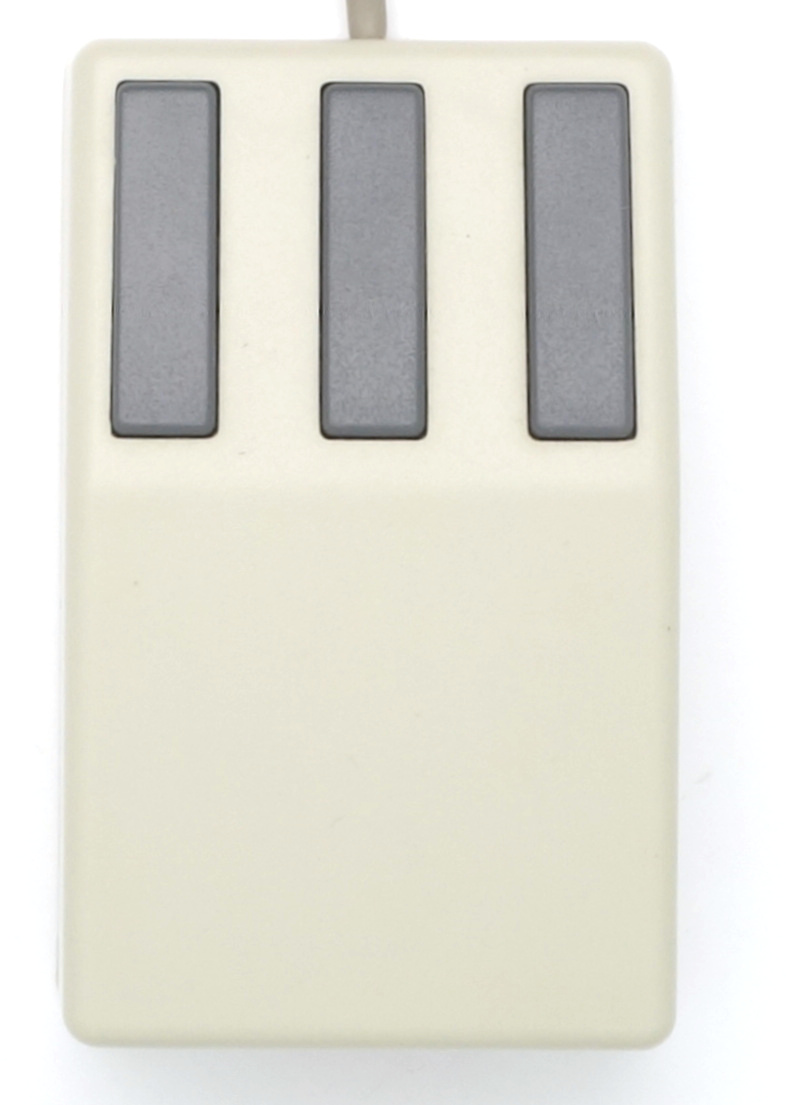
\includegraphics[scale=0.75]{1987_genius_gm5_mouse/top_30.jpg}
    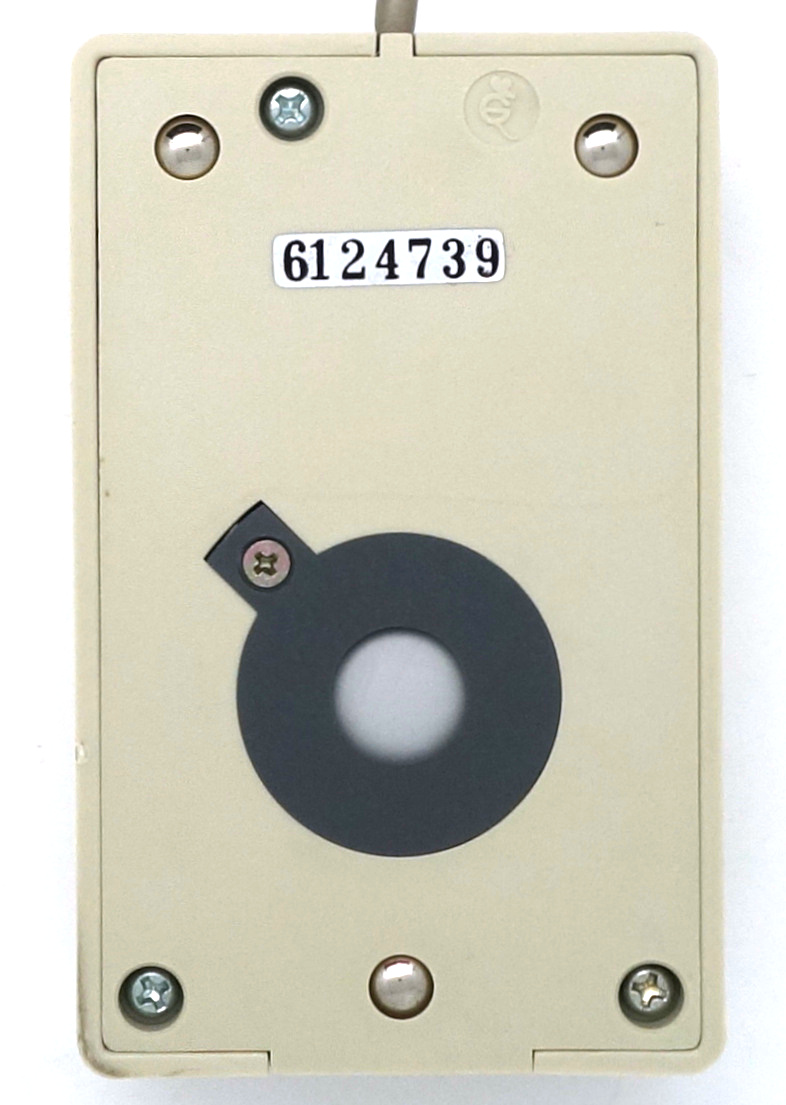
\includegraphics[scale=0.75]{1987_genius_gm5_mouse/bottom_30.jpg}
    \caption{Genius GM-5, вид сверху и снизу}
    \label{fig:GM5MouseTopAndBottom}
\end{figure}

Корпус имеет размер, типичный для первой половины 1980-х годов, и не демонстрирует никакой идентификации модели мыши. Только металлическая табличка, расположенная на ближнем к пользователю торце, имеет надпись <<Genius Mouse>> с вписанным логотипом Genius (рис. \ref{fig:GM5MousePic}, \ref{fig:GM5MouseSize}). Следует также отметить, что мышь GM-5 выпускалась в течение достаточно продолжительного времени, и известны экземпляры GM-5 в более новом корпусе "--- том, в котором появились модели  GM-6 и GM-6000 \cite{commodore}. Смена <<старого>> корпуса на <<новый>> в мышах Genius происходила постепенно: как минимум, в обновленном корпусе можно встретить также модели GM-3a (последовательная мышь, получающая питание от клавиатуры) и GM-4. Отсутствие чёткой идентификации модели мыши на корпусах позволяло KYE Systems использовать такие варианты корпуса, какие получалось, и даже чередовать их.

\begin{figure}[h]
    \centering
    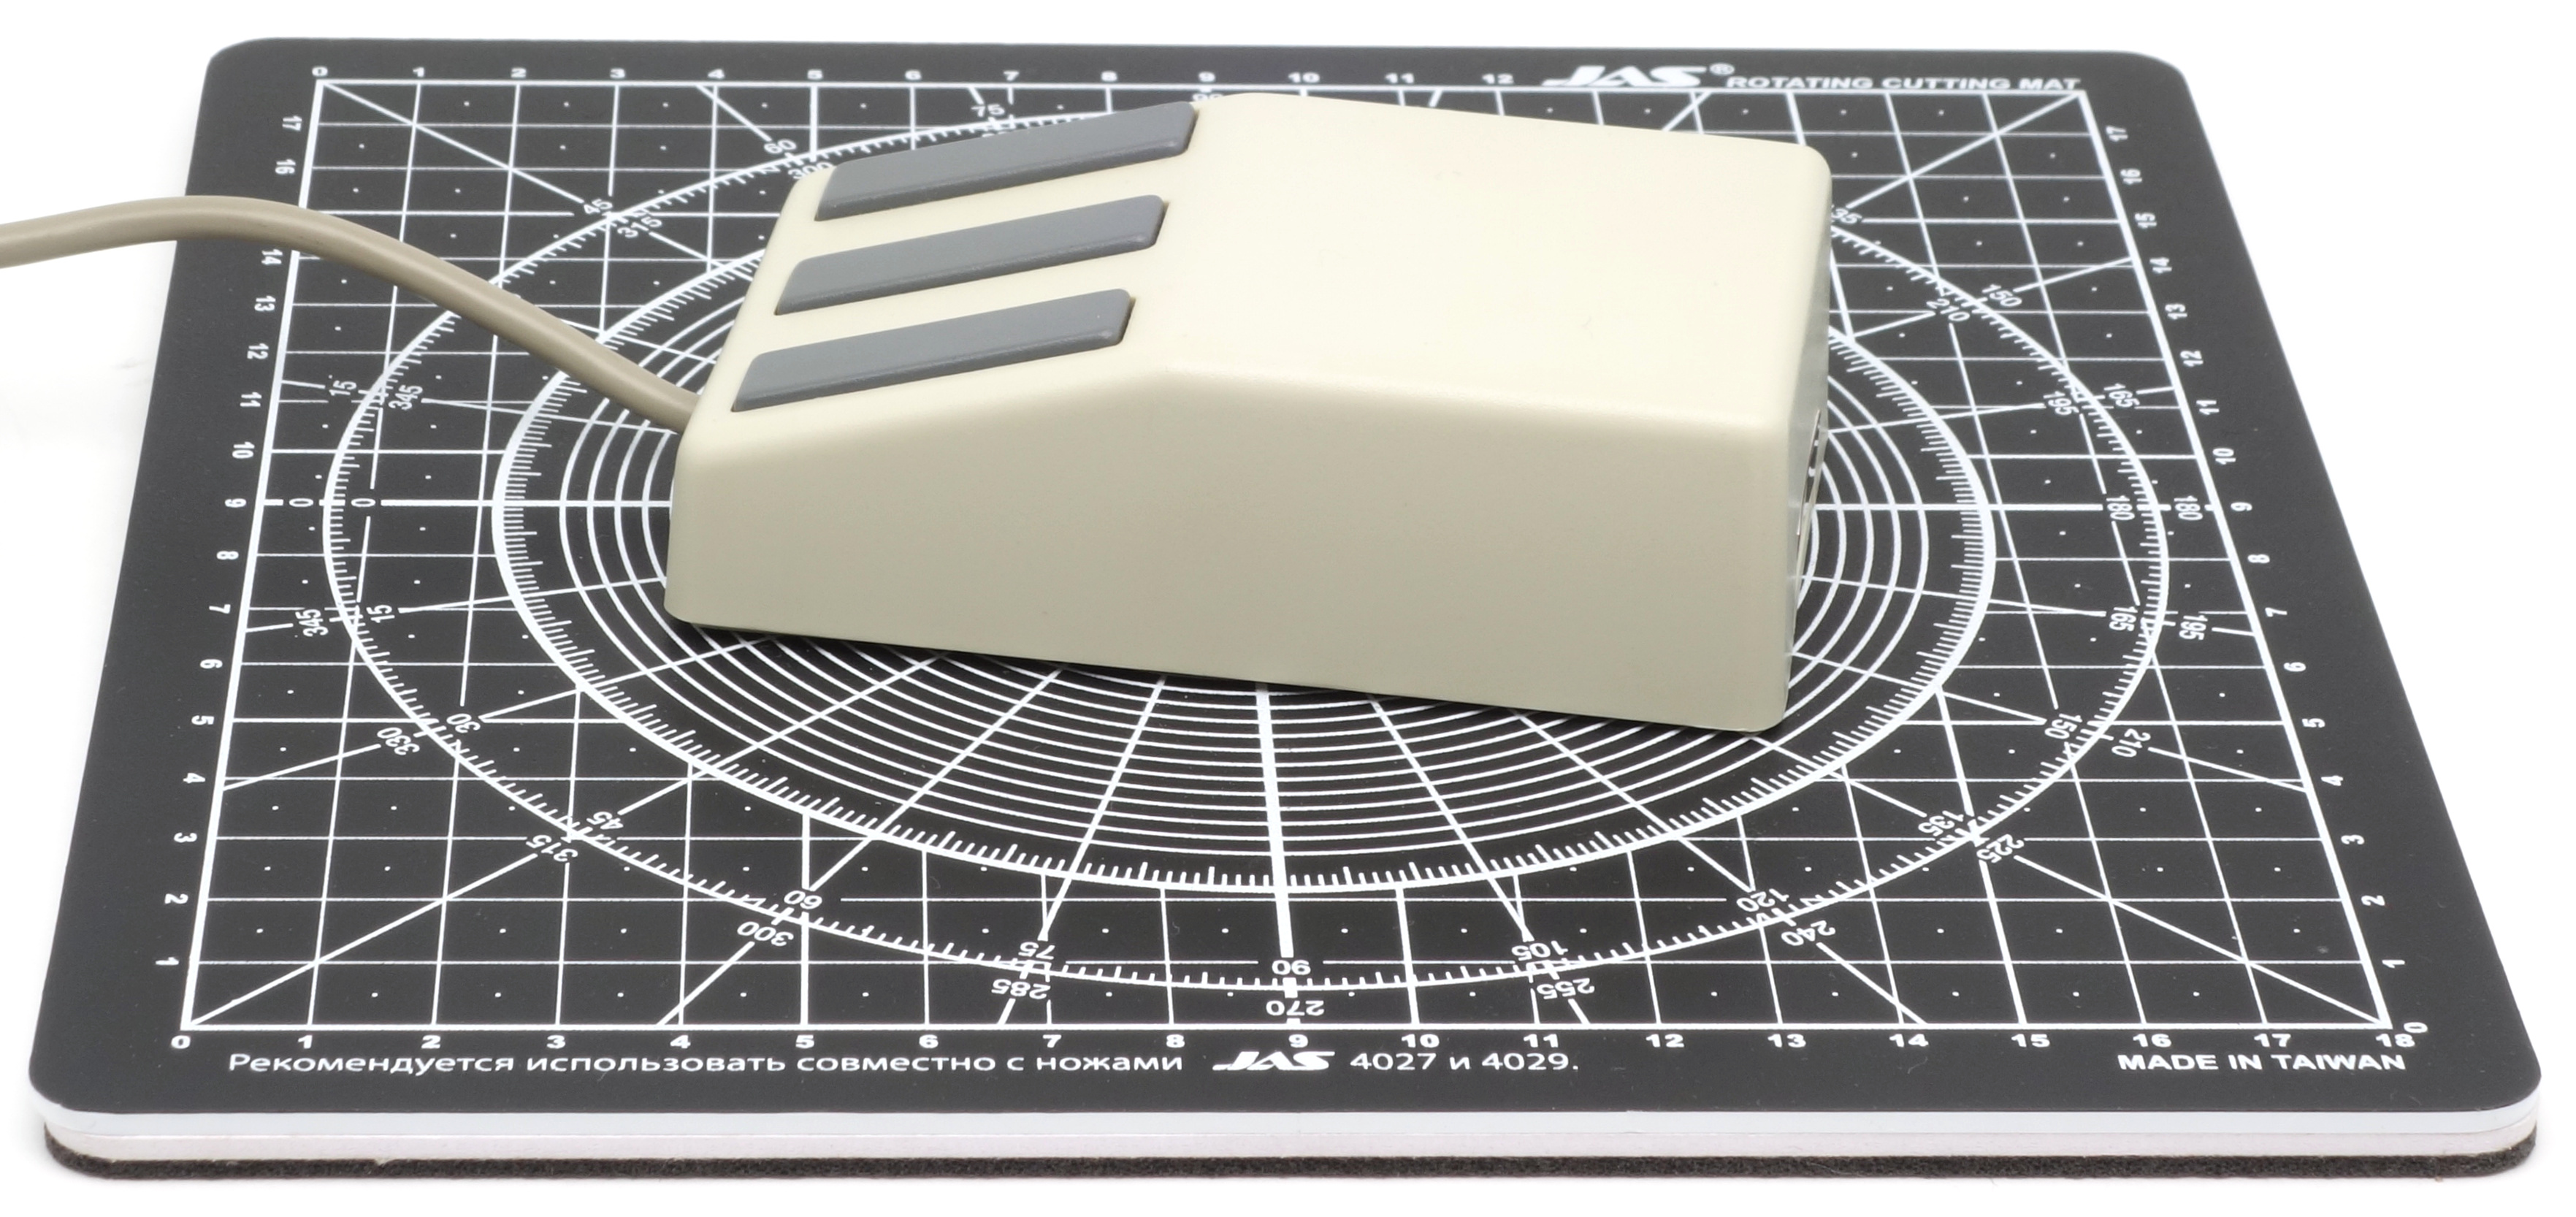
\includegraphics[scale=0.51]{1987_genius_gm5_mouse/size_30.jpg}
    \caption{Genius GM-5 на размерном коврике с шагом сетки 1~см}
    \label{fig:GM5MouseSize}
\end{figure}

В плане эргономики мышь GM-5 не может похвастаться существенными достоинствами. Пользовательский опыт очевидно страдает от суровой прямоугольности корпуса, с учетом того, что он имеет значительную высоту и не может обеспечить существенной поддержки ладони (рис. \ref{fig:GM5MouseHand}).

\begin{figure}[h]
    \centering
    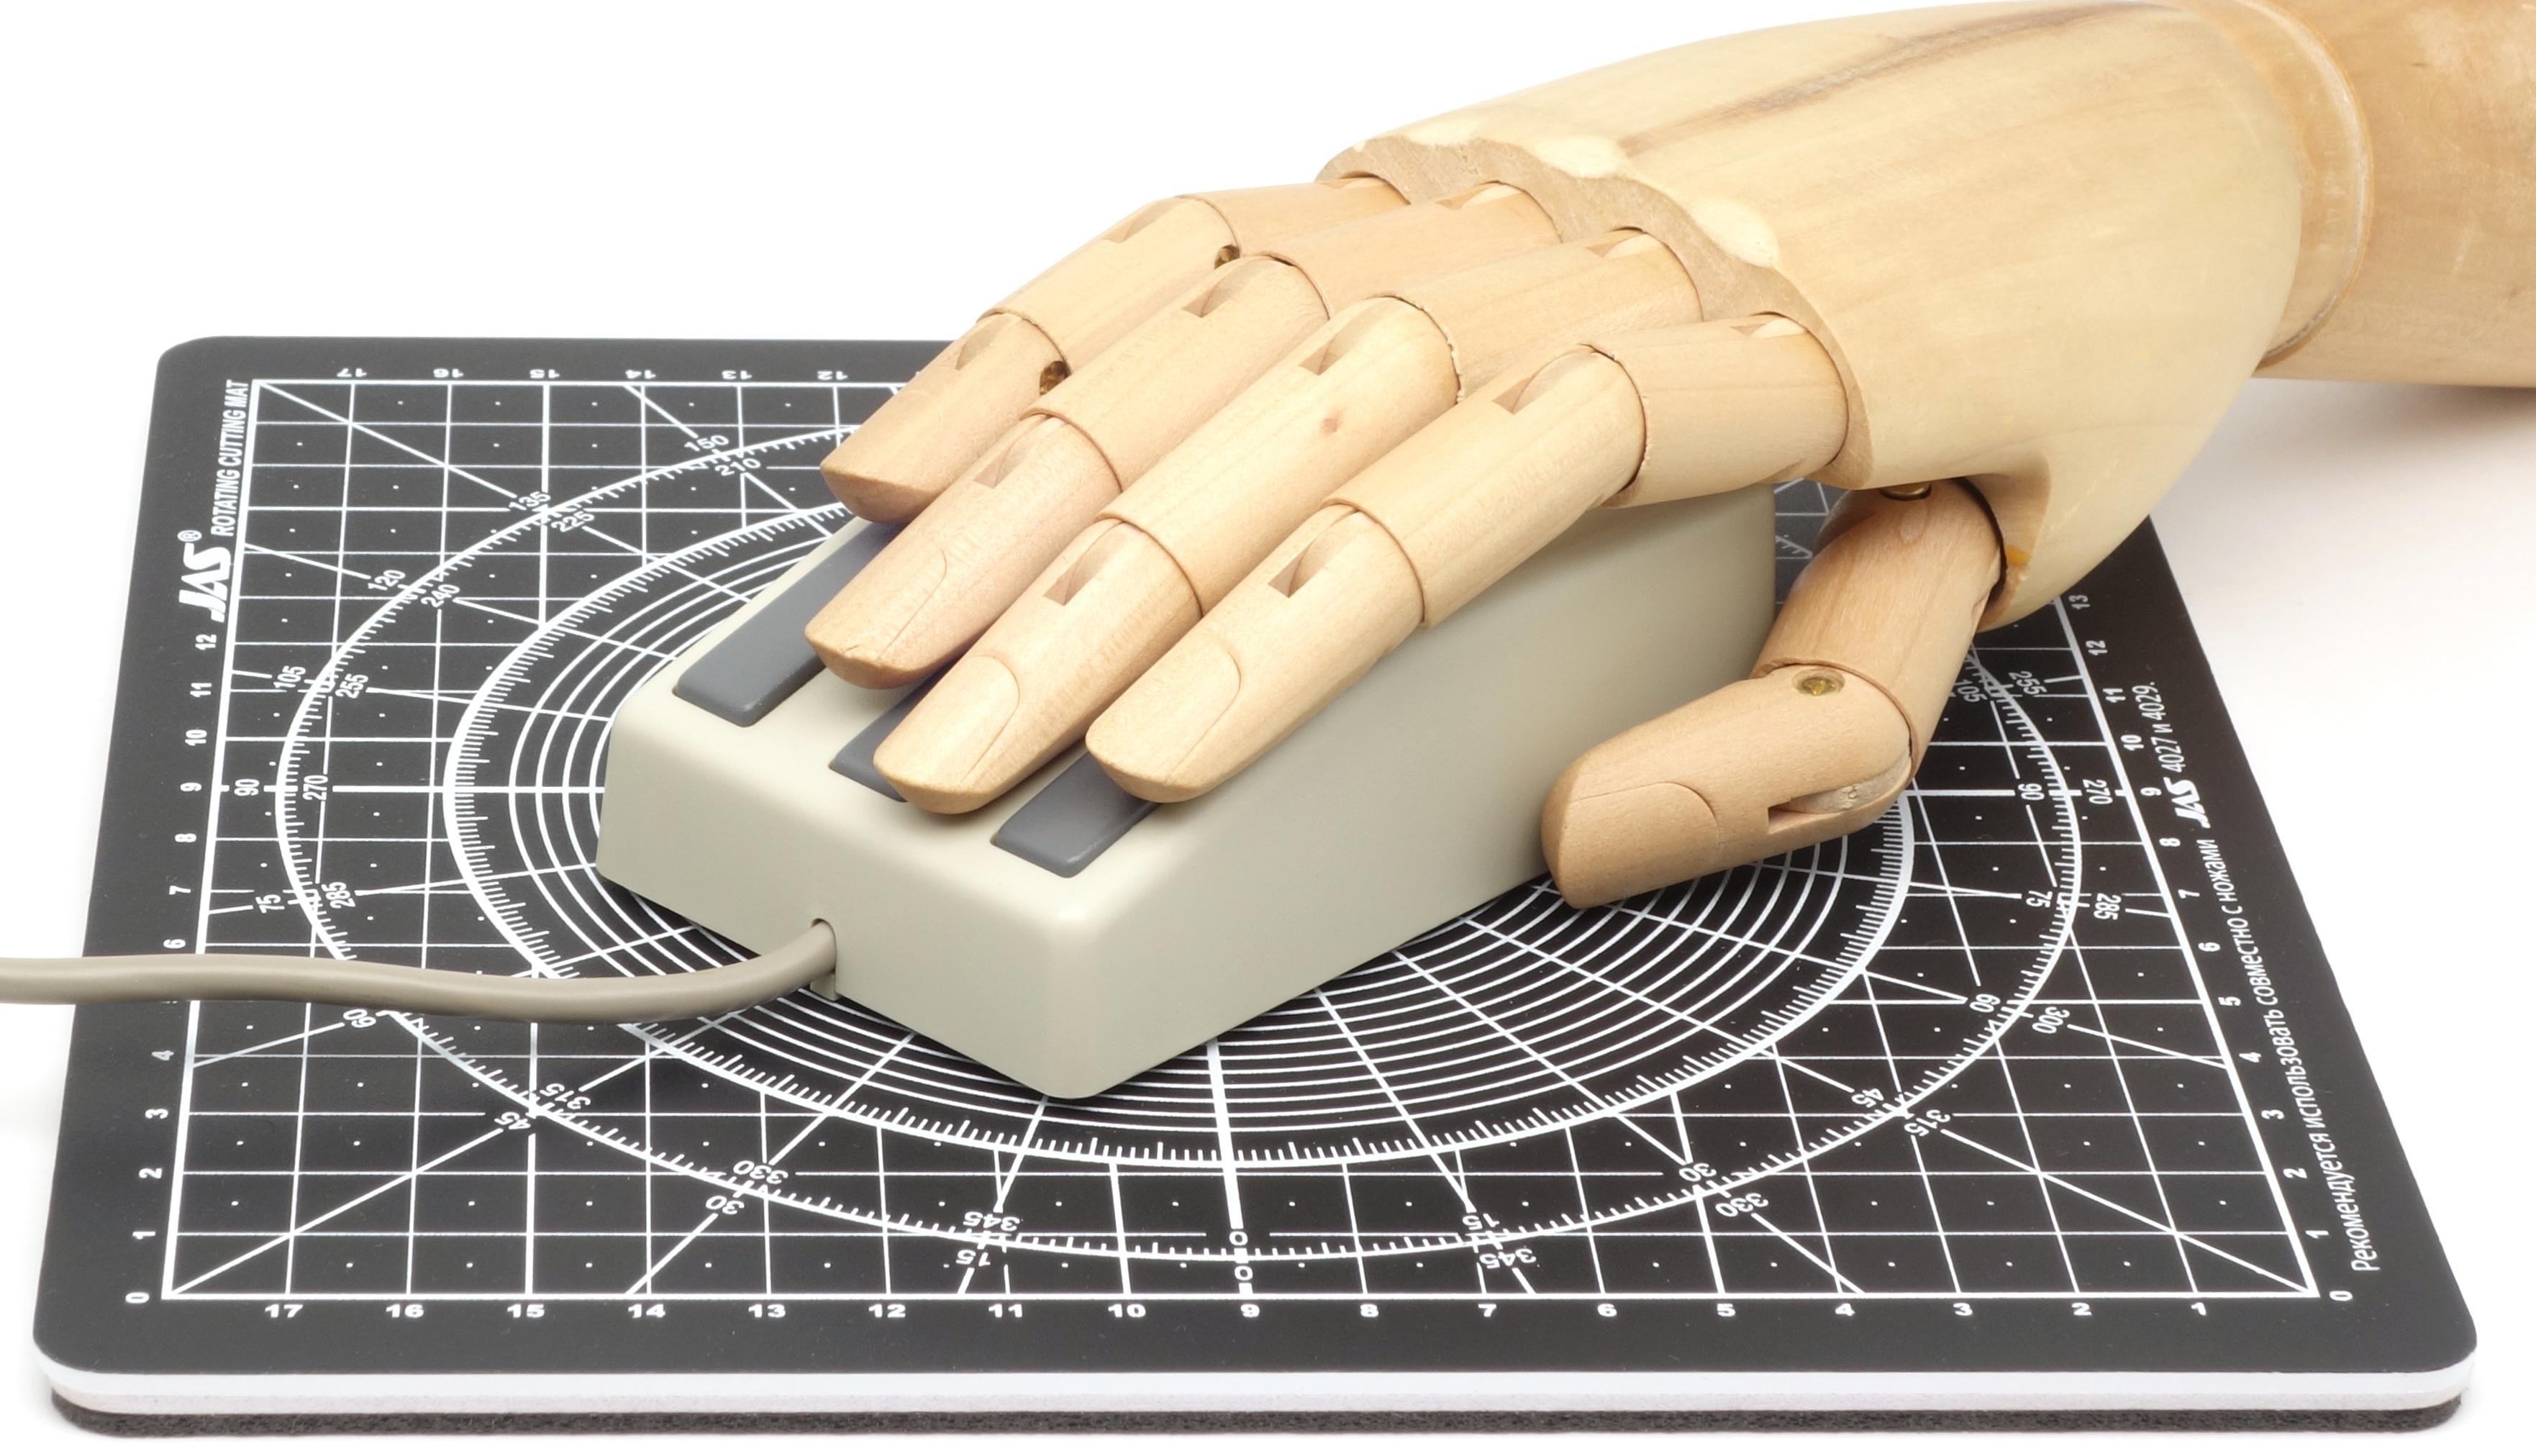
\includegraphics[scale=0.51]{1987_genius_gm5_mouse/hand_30.jpg}
    \caption{Genius GM-5 с моделью руки человека}
    \label{fig:GM5MouseHand}
\end{figure}

Внутреннее устройство мыши показано на рисунке \ref{fig:GM5MouseInside}. Как можно видеть, она представляет собой оптомеханическую конструкцию, типичную для второй половины или конца 80-х годов: с массивным пластмассовым обрамлением, закрывающим большую часть печатной платы, и достаточно долговечными латунными роликами.

 \begin{figure}[h]
    \centering
    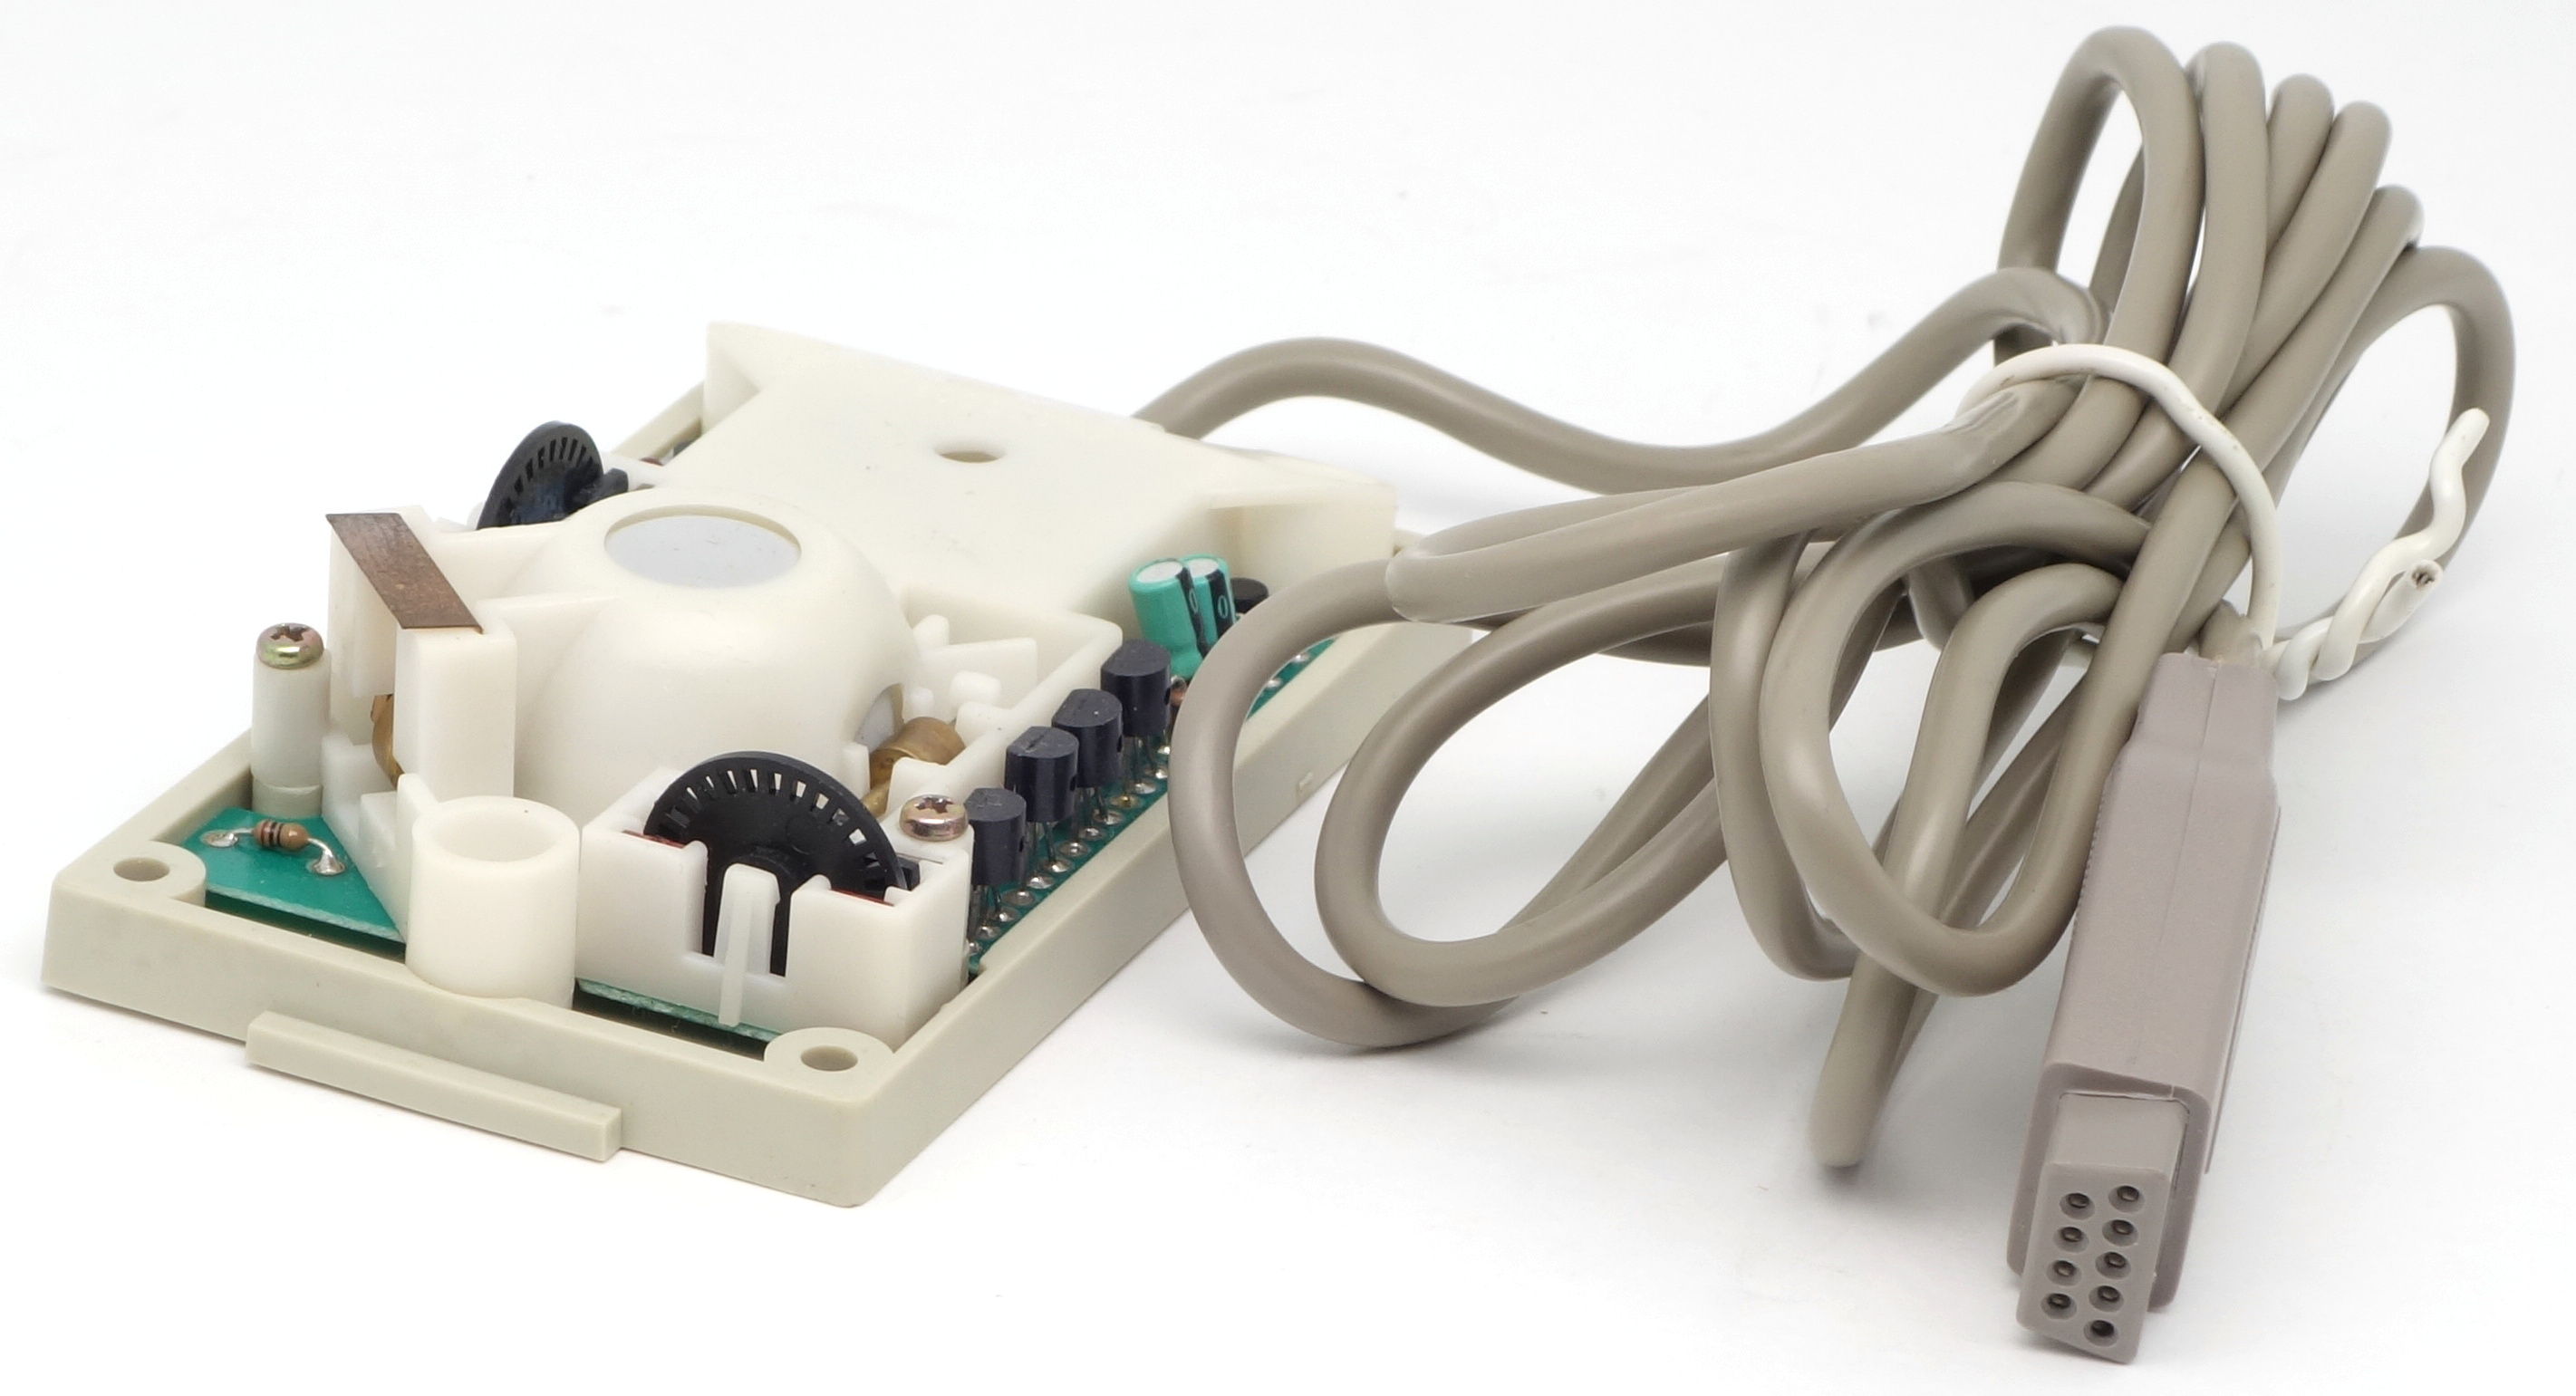
\includegraphics[scale=0.65]{1987_genius_gm5_mouse/inside_30.jpg}
    \caption{Genius GM-5 в разобранном виде}
    \label{fig:GM5MouseInside}
\end{figure}



\begin{thebibliography}{9}
\bibitem {armadale} Mouse - Genius for Commodore 64 | Collections WA \url{https://collectionswa.net.au/items/c38b1405-001b-454e-8b98-e93576187449}
\bibitem {YourComputer} Can Meet All Your Needs. PC/XT/AT. Peripherals \& PC Mouse (adv.) // Your Computer, March 1986. -- P. 24 \url{https://archive.org/details/1986.03-best-buys-ledger-masters/page/24/mode/2up}
\bibitem {commodore} Commodore Info Page - Joystick: Genius Mouse GM-5 [en]. \url{https://www.commodore-info.com/joystick/item/genius_mouse/en/desktop}
\end{thebibliography}
\end{document}
